% Created by tikzDevice version 0.12.3.1 on 2023-05-10 22:34:58
% !TEX encoding = UTF-8 Unicode
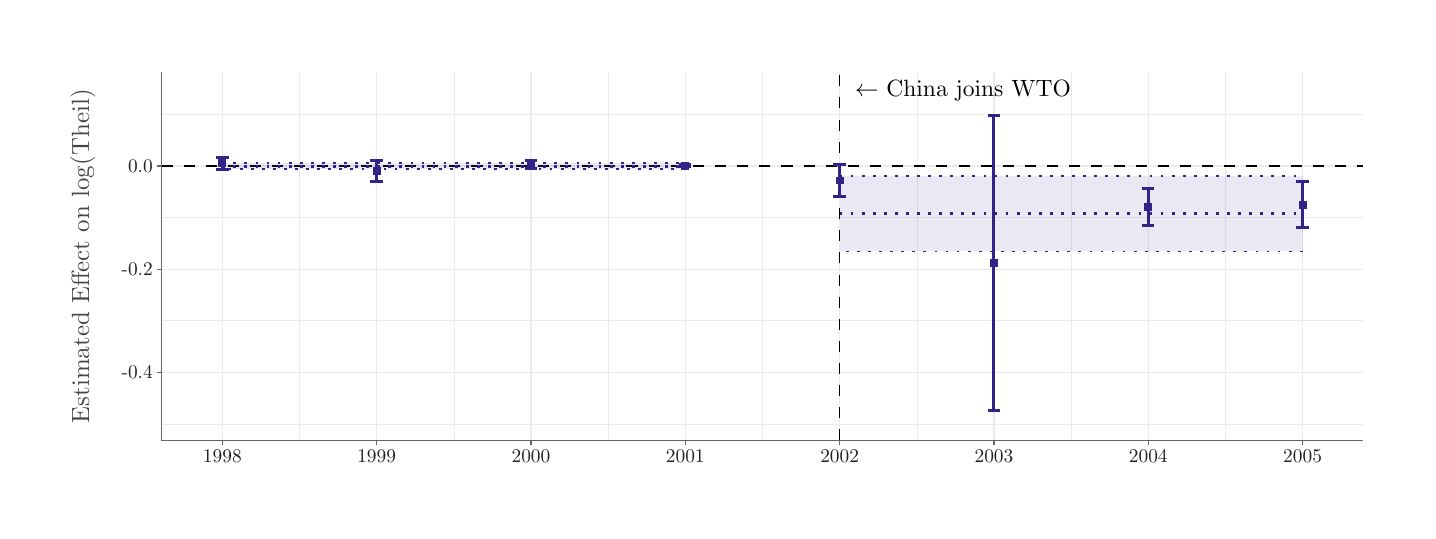
\begin{tikzpicture}[x=1pt,y=1pt]
\definecolor{fillColor}{RGB}{255,255,255}
\path[use as bounding box,fill=fillColor,fill opacity=0.00] (0,0) rectangle (498.66,174.53);
\begin{scope}
\path[clip] (  0.00,  0.00) rectangle (498.66,174.53);
\definecolor{fillColor}{RGB}{255,255,255}

\path[fill=fillColor] (  0.00,  0.00) rectangle (498.66,174.53);
\end{scope}
\begin{scope}
\path[clip] ( 48.37, 25.33) rectangle (482.66,158.53);
\definecolor{fillColor}{RGB}{255,255,255}

\path[fill=fillColor] ( 48.37, 25.33) rectangle (482.66,158.53);
\definecolor{drawColor}{gray}{0.92}

\path[draw=drawColor,line width= 0.2pt,line join=round] ( 48.37, 31.39) --
	(482.66, 31.39);

\path[draw=drawColor,line width= 0.2pt,line join=round] ( 48.37, 68.65) --
	(482.66, 68.65);

\path[draw=drawColor,line width= 0.2pt,line join=round] ( 48.37,105.90) --
	(482.66,105.90);

\path[draw=drawColor,line width= 0.2pt,line join=round] ( 48.37,143.16) --
	(482.66,143.16);

\path[draw=drawColor,line width= 0.2pt,line join=round] ( 98.22, 25.33) --
	( 98.22,158.53);

\path[draw=drawColor,line width= 0.2pt,line join=round] (153.99, 25.33) --
	(153.99,158.53);

\path[draw=drawColor,line width= 0.2pt,line join=round] (209.75, 25.33) --
	(209.75,158.53);

\path[draw=drawColor,line width= 0.2pt,line join=round] (265.52, 25.33) --
	(265.52,158.53);

\path[draw=drawColor,line width= 0.2pt,line join=round] (321.28, 25.33) --
	(321.28,158.53);

\path[draw=drawColor,line width= 0.2pt,line join=round] (377.04, 25.33) --
	(377.04,158.53);

\path[draw=drawColor,line width= 0.2pt,line join=round] (432.81, 25.33) --
	(432.81,158.53);

\path[draw=drawColor,line width= 0.4pt,line join=round] ( 48.37, 50.02) --
	(482.66, 50.02);

\path[draw=drawColor,line width= 0.4pt,line join=round] ( 48.37, 87.27) --
	(482.66, 87.27);

\path[draw=drawColor,line width= 0.4pt,line join=round] ( 48.37,124.53) --
	(482.66,124.53);

\path[draw=drawColor,line width= 0.4pt,line join=round] ( 70.34, 25.33) --
	( 70.34,158.53);

\path[draw=drawColor,line width= 0.4pt,line join=round] (126.10, 25.33) --
	(126.10,158.53);

\path[draw=drawColor,line width= 0.4pt,line join=round] (181.87, 25.33) --
	(181.87,158.53);

\path[draw=drawColor,line width= 0.4pt,line join=round] (237.63, 25.33) --
	(237.63,158.53);

\path[draw=drawColor,line width= 0.4pt,line join=round] (293.40, 25.33) --
	(293.40,158.53);

\path[draw=drawColor,line width= 0.4pt,line join=round] (349.16, 25.33) --
	(349.16,158.53);

\path[draw=drawColor,line width= 0.4pt,line join=round] (404.93, 25.33) --
	(404.93,158.53);

\path[draw=drawColor,line width= 0.4pt,line join=round] (460.69, 25.33) --
	(460.69,158.53);
\definecolor{drawColor}{RGB}{0,0,0}

\path[draw=drawColor,line width= 0.6pt,dash pattern=on 4pt off 4pt ,line join=round] ( 48.37,124.53) -- (482.66,124.53);

\path[draw=drawColor,line width= 0.6pt,dash pattern=on 4pt off 4pt ,line join=round] (293.40, 25.33) -- (293.40,158.53);

\node[text=drawColor,anchor=base west,inner sep=0pt, outer sep=0pt, scale=  0.85] at (298.97,149.54) {$\leftarrow$ China joins WTO};
\definecolor{drawColor}{RGB}{51,34,136}

\path[draw=drawColor,line width= 1.1pt,line join=round] ( 68.11,127.69) --
	( 72.57,127.69);

\path[draw=drawColor,line width= 1.1pt,line join=round] ( 70.34,127.69) --
	( 70.34,123.35);

\path[draw=drawColor,line width= 1.1pt,line join=round] ( 68.11,123.35) --
	( 72.57,123.35);

\path[draw=drawColor,line width= 1.1pt,line join=round] (123.87,126.67) --
	(128.34,126.67);

\path[draw=drawColor,line width= 1.1pt,line join=round] (126.10,126.67) --
	(126.10,118.83);

\path[draw=drawColor,line width= 1.1pt,line join=round] (123.87,118.83) --
	(128.34,118.83);

\path[draw=drawColor,line width= 1.1pt,line join=round] (179.64,126.65) --
	(184.10,126.65);

\path[draw=drawColor,line width= 1.1pt,line join=round] (181.87,126.65) --
	(181.87,123.74);

\path[draw=drawColor,line width= 1.1pt,line join=round] (179.64,123.74) --
	(184.10,123.74);

\path[draw=drawColor,line width= 1.1pt,line join=round] (235.40,124.96) --
	(239.86,124.96);

\path[draw=drawColor,line width= 1.1pt,line join=round] (237.63,124.96) --
	(237.63,124.37);

\path[draw=drawColor,line width= 1.1pt,line join=round] (235.40,124.37) --
	(239.86,124.37);

\path[draw=drawColor,line width= 1.1pt,line join=round] (291.17,124.99) --
	(295.63,124.99);

\path[draw=drawColor,line width= 1.1pt,line join=round] (293.40,124.99) --
	(293.40,113.62);

\path[draw=drawColor,line width= 1.1pt,line join=round] (291.17,113.62) --
	(295.63,113.62);

\path[draw=drawColor,line width= 1.1pt,line join=round] (346.93,142.90) --
	(351.39,142.90);

\path[draw=drawColor,line width= 1.1pt,line join=round] (349.16,142.90) --
	(349.16, 36.36);

\path[draw=drawColor,line width= 1.1pt,line join=round] (346.93, 36.36) --
	(351.39, 36.36);

\path[draw=drawColor,line width= 1.1pt,line join=round] (402.70,116.39) --
	(407.16,116.39);

\path[draw=drawColor,line width= 1.1pt,line join=round] (404.93,116.39) --
	(404.93,103.10);

\path[draw=drawColor,line width= 1.1pt,line join=round] (402.70,103.10) --
	(407.16,103.10);

\path[draw=drawColor,line width= 1.1pt,line join=round] (458.46,118.95) --
	(462.92,118.95);

\path[draw=drawColor,line width= 1.1pt,line join=round] (460.69,118.95) --
	(460.69,102.22);

\path[draw=drawColor,line width= 1.1pt,line join=round] (458.46,102.22) --
	(462.92,102.22);
\definecolor{fillColor}{RGB}{51,34,136}

\path[fill=fillColor] ( 68.91,124.09) --
	( 71.77,124.09) --
	( 71.77,126.95) --
	( 68.91,126.95) --
	cycle;

\path[fill=fillColor] (124.68,121.32) --
	(127.53,121.32) --
	(127.53,124.18) --
	(124.68,124.18) --
	cycle;

\path[fill=fillColor] (180.44,123.77) --
	(183.30,123.77) --
	(183.30,126.62) --
	(180.44,126.62) --
	cycle;

\path[fill=fillColor] (236.21,123.24) --
	(239.06,123.24) --
	(239.06,126.09) --
	(236.21,126.09) --
	cycle;

\path[fill=fillColor] (291.97,117.88) --
	(294.82,117.88) --
	(294.82,120.73) --
	(291.97,120.73) --
	cycle;

\path[fill=fillColor] (347.74, 88.21) --
	(350.59, 88.21) --
	(350.59, 91.06) --
	(347.74, 91.06) --
	cycle;

\path[fill=fillColor] (403.50,108.32) --
	(406.35,108.32) --
	(406.35,111.17) --
	(403.50,111.17) --
	cycle;

\path[fill=fillColor] (459.27,109.16) --
	(462.12,109.16) --
	(462.12,112.01) --
	(459.27,112.01) --
	cycle;
\definecolor{fillColor}{RGB}{51,34,136}

\path[fill=fillColor,fill opacity=0.10] (293.40,120.96) --
	(460.69,120.96) --
	(460.69, 93.67) --
	(293.40, 93.67) --
	cycle;

\path[draw=drawColor,line width= 0.6pt,dash pattern=on 1pt off 3pt ,line join=round] (293.40,120.96) --
	(460.69,120.96);

\path[draw=drawColor,line width= 0.6pt,dash pattern=on 1pt off 3pt ,line join=round] (460.69, 93.67) --
	(293.40, 93.67);

\path[fill=fillColor,fill opacity=0.10] ( 70.34,125.71) --
	(237.63,125.71) --
	(237.63,123.35) --
	( 70.34,123.35) --
	cycle;

\path[draw=drawColor,line width= 0.6pt,dash pattern=on 1pt off 3pt ,line join=round] ( 70.34,125.71) --
	(237.63,125.71);

\path[draw=drawColor,line width= 0.6pt,dash pattern=on 1pt off 3pt ,line join=round] (237.63,123.35) --
	( 70.34,123.35);

\path[draw=drawColor,line width= 1.1pt,dash pattern=on 1pt off 3pt ,line join=round] (293.40,107.32) --
	(460.69,107.32);

\path[draw=drawColor,line width= 1.1pt,dash pattern=on 1pt off 3pt ,line join=round] ( 70.34,124.53) --
	(237.63,124.53);
\end{scope}
\begin{scope}
\path[clip] (  0.00,  0.00) rectangle (498.66,174.53);
\definecolor{drawColor}{gray}{0.40}

\path[draw=drawColor,line width= 0.4pt,line join=round] ( 48.37, 25.33) --
	( 48.37,158.53);
\end{scope}
\begin{scope}
\path[clip] (  0.00,  0.00) rectangle (498.66,174.53);
\definecolor{drawColor}{gray}{0.13}

\node[text=drawColor,anchor=base east,inner sep=0pt, outer sep=0pt, scale=  0.70] at ( 45.22, 47.61) {-0.4};

\node[text=drawColor,anchor=base east,inner sep=0pt, outer sep=0pt, scale=  0.70] at ( 45.22, 84.86) {-0.2};

\node[text=drawColor,anchor=base east,inner sep=0pt, outer sep=0pt, scale=  0.70] at ( 45.22,122.12) {0.0};
\end{scope}
\begin{scope}
\path[clip] (  0.00,  0.00) rectangle (498.66,174.53);
\definecolor{drawColor}{gray}{0.40}

\path[draw=drawColor,line width= 0.4pt,line join=round] ( 46.62, 50.02) --
	( 48.37, 50.02);

\path[draw=drawColor,line width= 0.4pt,line join=round] ( 46.62, 87.27) --
	( 48.37, 87.27);

\path[draw=drawColor,line width= 0.4pt,line join=round] ( 46.62,124.53) --
	( 48.37,124.53);
\end{scope}
\begin{scope}
\path[clip] (  0.00,  0.00) rectangle (498.66,174.53);
\definecolor{drawColor}{gray}{0.40}

\path[draw=drawColor,line width= 0.4pt,line join=round] ( 48.37, 25.33) --
	(482.66, 25.33);
\end{scope}
\begin{scope}
\path[clip] (  0.00,  0.00) rectangle (498.66,174.53);
\definecolor{drawColor}{gray}{0.40}

\path[draw=drawColor,line width= 0.4pt,line join=round] ( 70.34, 23.58) --
	( 70.34, 25.33);

\path[draw=drawColor,line width= 0.4pt,line join=round] (126.10, 23.58) --
	(126.10, 25.33);

\path[draw=drawColor,line width= 0.4pt,line join=round] (181.87, 23.58) --
	(181.87, 25.33);

\path[draw=drawColor,line width= 0.4pt,line join=round] (237.63, 23.58) --
	(237.63, 25.33);

\path[draw=drawColor,line width= 0.4pt,line join=round] (293.40, 23.58) --
	(293.40, 25.33);

\path[draw=drawColor,line width= 0.4pt,line join=round] (349.16, 23.58) --
	(349.16, 25.33);

\path[draw=drawColor,line width= 0.4pt,line join=round] (404.93, 23.58) --
	(404.93, 25.33);

\path[draw=drawColor,line width= 0.4pt,line join=round] (460.69, 23.58) --
	(460.69, 25.33);
\end{scope}
\begin{scope}
\path[clip] (  0.00,  0.00) rectangle (498.66,174.53);
\definecolor{drawColor}{gray}{0.13}

\node[text=drawColor,anchor=base,inner sep=0pt, outer sep=0pt, scale=  0.70] at ( 70.34, 17.36) {1998};

\node[text=drawColor,anchor=base,inner sep=0pt, outer sep=0pt, scale=  0.70] at (126.10, 17.36) {1999};

\node[text=drawColor,anchor=base,inner sep=0pt, outer sep=0pt, scale=  0.70] at (181.87, 17.36) {2000};

\node[text=drawColor,anchor=base,inner sep=0pt, outer sep=0pt, scale=  0.70] at (237.63, 17.36) {2001};

\node[text=drawColor,anchor=base,inner sep=0pt, outer sep=0pt, scale=  0.70] at (293.40, 17.36) {2002};

\node[text=drawColor,anchor=base,inner sep=0pt, outer sep=0pt, scale=  0.70] at (349.16, 17.36) {2003};

\node[text=drawColor,anchor=base,inner sep=0pt, outer sep=0pt, scale=  0.70] at (404.93, 17.36) {2004};

\node[text=drawColor,anchor=base,inner sep=0pt, outer sep=0pt, scale=  0.70] at (460.69, 17.36) {2005};
\end{scope}
\begin{scope}
\path[clip] (  0.00,  0.00) rectangle (498.66,174.53);
\definecolor{drawColor}{gray}{0.27}

\node[text=drawColor,rotate= 90.00,anchor=base,inner sep=0pt, outer sep=0pt, scale=  0.90] at ( 22.20, 91.93) {Estimated Effect on $\log($Theil$)$};
\end{scope}
\end{tikzpicture}
